\noindent L’apprentissage profond est un sous-domaine de celui de l'apprentissage machine qui est un sous-domaine de celui de l'intelligence artificielle (figure \ref{fig:ia_ml_ap}). 
\vspace{0.5\baselineskip}
\\
\noindent Les concepts de l'\lowercase{\acrlong{ia}} (AI) existent depuis les années 1950 \parencite{chollet_deep_2018, alom_history_2018}, et ont continué à se développer par vague, jusqu'à leur nouvelle popularité des 15 dernières années. En effet, trois raisons principales ont permis à ce domaine de renaitre de nouveau \parencite[p.~20]{chollet_deep_2018}: 1) la capacité et la puissance des machines; 2) des jeux de données plus larges; 3) des algorithmes plus avancés. Les deux moments clés, preuves de cette renaissance, sont: 1) la possibilité d'entrainer des architectures de réseaux de neurones profonds (DNN) (2006) \parencite[p.~6]{alom_history_2018}; et 2) l'architecture du réseau de neurones convolutionels AlexNet permet de gagner le challenge ImageNet contre les approches traditionnelles \parencite[p.~11]{alom_history_2018}. 
\begin{figure}[H]
   \centering
   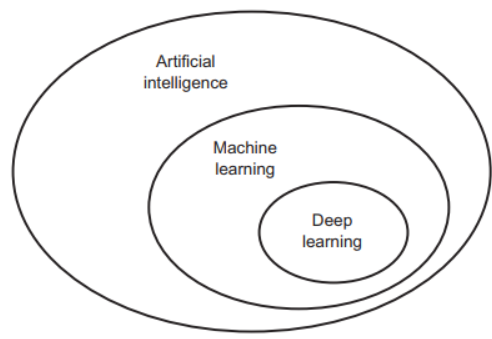
\includegraphics[width=0.5\textwidth]{Deep_Learning_with_Python.pdf}
   \caption[Relation entre \acrlong{ia}, \acrlong{am} et \acrlong{ap}]{Relation entre \acrlong{ia}, \acrlong{am} et \acrlong{ap} \parencite[p.~4]{chollet_deep_2018}}
   \label{fig:ia_ml_ap}
\end{figure}
\noindent La détection d'objets en temps réel est de plus en plus précise et efficace depuis que les performances des systèmes informatisés permettent l'exécution d'algorithmes exigeants, en majeure partie depuis l'utilisation des processeurs graphiques "\acrshort{gpu}" \parencite{chong_real-time_1992, dettmers_deep_2015, beam_deep_2017, jiaconda_concise_2019, zheng_real-time_2020, kurenkov_brief_2015}. 
\vspace{0.5\baselineskip}
\\
\noindent Les réseaux de neurones ont rapidement progressé depuis 2012 \parencite{beam_deep_2017}, permettant d'offrir des alternatives aux solutions de détection et de classifications tel que les algorithmes SIFT et HOG \parencite{pathak_architecturally_2019}. Les réseaux de neurones pleinement connectés ("\acrshort{fcn}" en anglais, pour "\acrlong{fcn-en}") sont les derniers à avoir émergé et représente l'état de l'art \parencite{zheng_real-time_2020} et à profiter au domaine de la vision et de la détection d'objets \parencite{nguyen_mavnet_2019, zheng_real-time_2020}. En 2016 \parencite[p.~14]{alom_history_2018}, l'architecture \acrshort{fcn} a permis aux tâches réservées à la segmentation d'images d'être plus efficace que les méthodes traditionnelles de la vision par ordinateur. Cette nouvelle méthode s'applique désormais à tous les domaines connexes à l'analyse d'images, tels que l'imagerie médicale, la conduite autonome de véhicules, la robotique, la télédétection d'images satellites, la sécurité par caméra vidéo, l'agriculture de haute précision. Aujourd'hui, elle peut s'exécuter en temps réel sur des systèmes embarqués proche des données. 
\vspace{0.5\baselineskip}
\\
\noindent La segmentation sémantique d'images ou de vidéos (figure \ref{fig:semantic_segmentation_vs_others}) est une technique de télédétection du domaine de la vision par ordinateur. Elle permet de délimiter (segmenter) différentes parties (sémantique) d'une image. Les méthodes de segmentation ont été améliorées ces dernières années par les récentes avancées dans le domaine de l'apprentissage profond. 
\vspace{0.5\baselineskip}
\\
\noindent Les cadres de développemement d'application logicielle d'apprentissage profond les plus courants sont identifiées par \parencite{cornioley_integration_2018}. On peut préciser que celles les plus populaires à ce jour sont PyTorch, TensorFlow et Keras, et sont accessibles via le langage de programmation Python. Keras est une solution intéressante, car elle ajoute une couche d'abstraction à d'autres ( PyTorch, TensorFlow et Caffee), et donc est précurseur dans ce domaine où la simplification et l'accessibilité de la programmation sont recherchées. Une liste plus exhaustive est fournie par le projet communautaire \acrshort{onnx}\footnote{\url{https://onnx.ai/supported-tools}}.
\vspace{0.5\baselineskip}
\\
\noindent \acrshort{onnx} (\acrlong{onnx}) est un projet communautaire qui mets à disposition une plateforme applicative permettant de rendre interopérable, pour l'inférence, des architectures de réseaux de neurones conçues avec différentes plateformes applicatives d'apprentissage machine, tels que PyTorch et TensorFlow. Initié par Facebook en 2017\footnote{\url{https://en.wikipedia.org/wiki/Open_Neural_Network_Exchange}} et soutenue par l'ensemble des acteurs du domaine (IBM, AWS, Microsoft, NVIDIA, Intel, etc.)\footnote{\url{https://onnx.ai/about.html}}, elle est implémentée par NVIDIA dans la solution applicative du Jetson Nano pour l'inférence, et supporte donc des modèles personnalisés, tant qu'ils peuvent être convertis au format \acrshort{onnx}, peu importe la plateforme avec laquelle ils ont été conçus. Peu de références dans la littérature y font référence à ce jour\footnote{19 résultats dans SCOPUS le 8 mai 2021}.